\subsection{El núcleo de la mochila, módulo por módulo}
\label{sec:nucleo}

La mochila deja que el insecto explore solo y estimula lo mínimo. La política es una máquina de ocho estados que
avanza una vez por cuadro térmico, diez veces por segundo (figura~\ref{fig:fsm}), y tres reglas la distinguen de
un control remoto: la espera que se duplica si el insecto no responde, los giros al azar que lo despegan de las
paredes~\cite{dirafzoon2017} y un presupuesto que limita los estímulos. La figura~\ref{fig:nucleo} muestra los
módulos; el recuadro punteado es lo que iría en el chip. En cada encabezado van el archivo y los elementos
lógicos (EL) y registros (R) que reporta Quartus.

\begin{figure}[!htb]
\centering
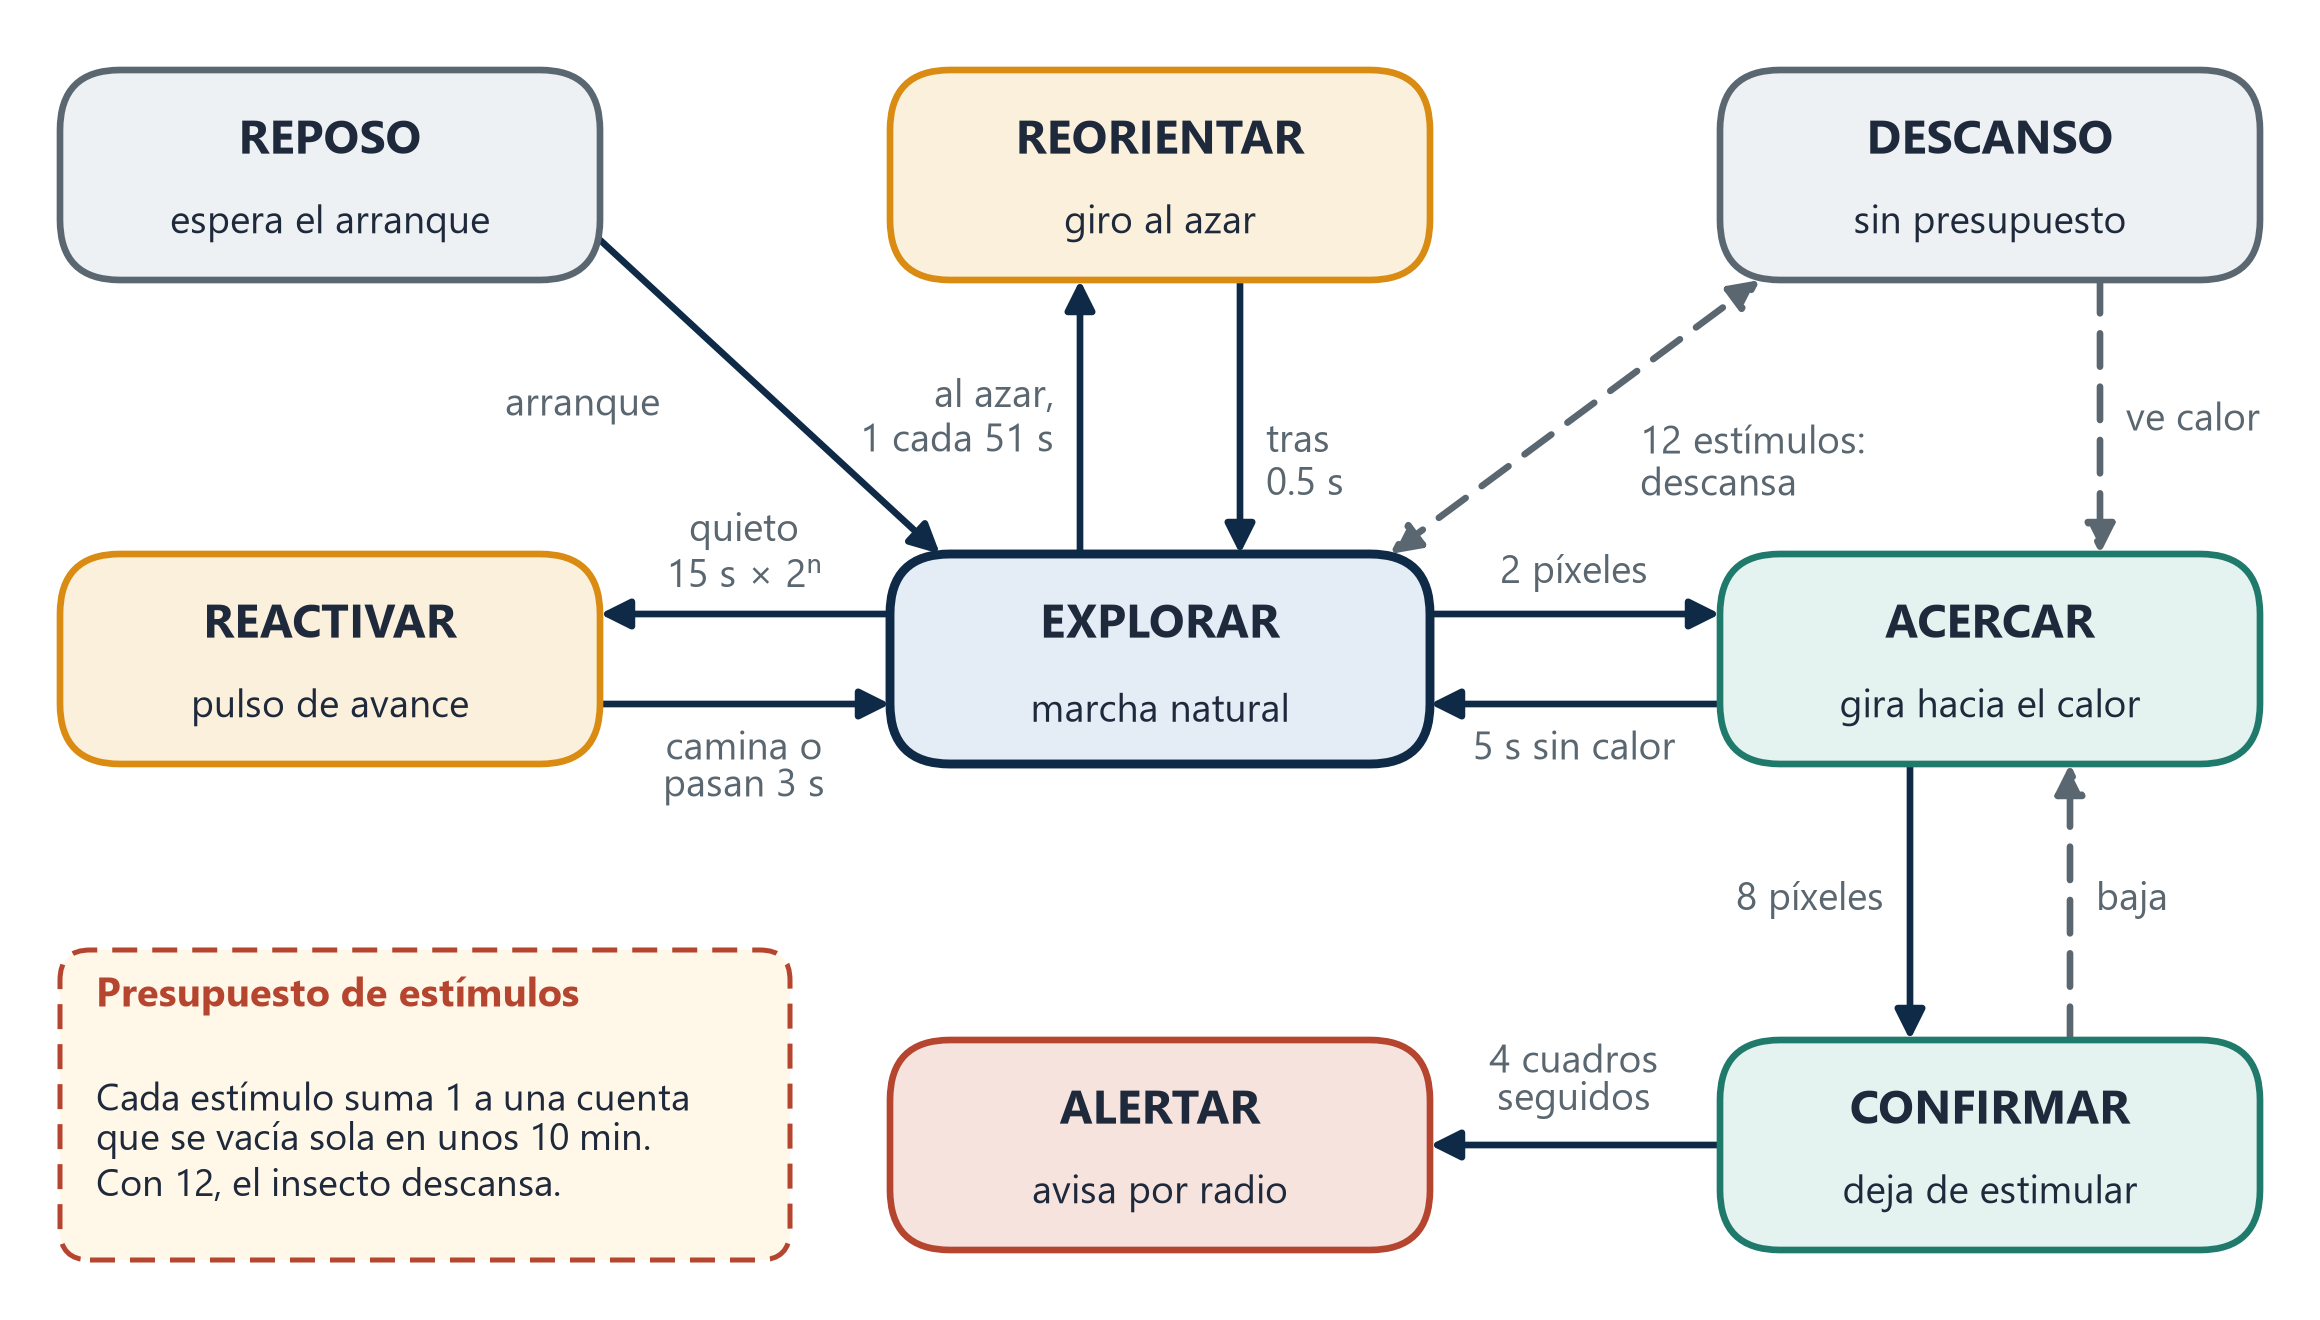
\includegraphics[width=0.80\textwidth]{figs/fsm_politica.png}
\caption{Máquina de estados de la política. Las flechas punteadas no producen estímulo.}
\label{fig:fsm}
\end{figure}

\begin{figure}[!htb]
\centering
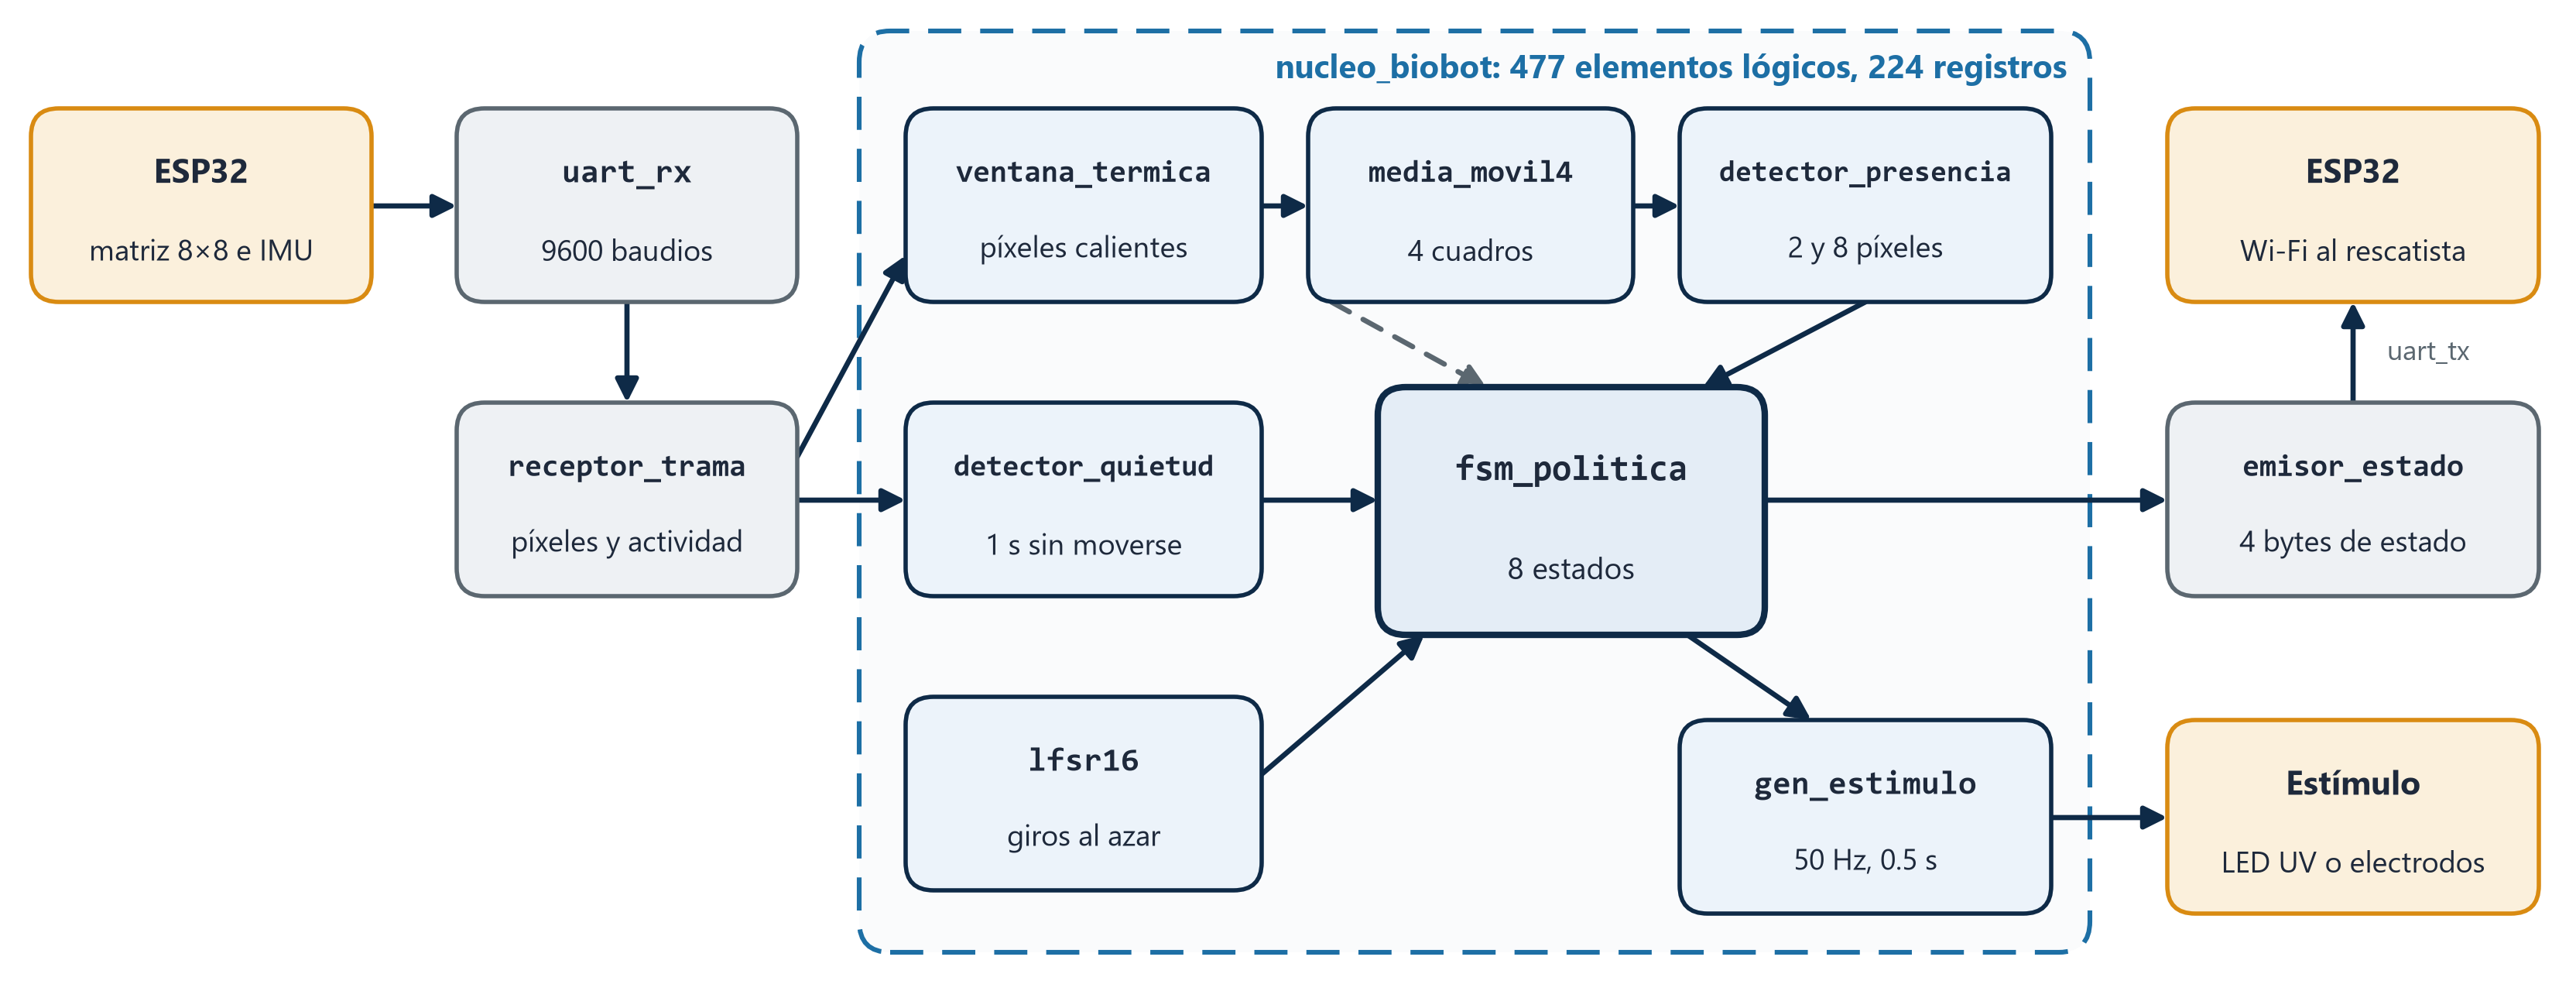
\includegraphics[width=\textwidth]{figs/nucleo_digital.png}
\caption{Módulos Verilog del núcleo y del enlace serie del prototipo.}
\label{fig:nucleo}
\end{figure}

\modulo{ventana\_termica}{hdl/ventana\_termica.v}{160 EL, 61 R}
Recibe la matriz píxel por píxel, un byte de 0.25~\textdegree C por cuenta con un pulso \sig{px\_valido}. Dos
comparadores revisan la ventana de piel ($T_{\min}\le T\le T_{\max}$, por omisión 112 y 152 cuentas, o sea 28 y
38~\textdegree C) y un tercero exige superar el fondo en 8 cuentas (2~\textdegree C); si los tres se cumplen, el
píxel es caliente. Tres contadores llevan el total, los de las columnas 0 a 2 y los de las columnas 5 a 7, y un
acumulador de 14 bits suma las temperaturas. Con \sig{px\_ultimo} cierra el cuadro: publica el conteo, el lado
que domina (01 izquierda, 10 derecha, 00 centro) y la media, que se obtiene con un corrimiento de 6 bits y sirve
de fondo para el cuadro siguiente. Los valores se calculan con el píxel actual ya sumado, así que todo cierra en
el mismo ciclo. El fondo arranca en 255: en el primer cuadro nada puede ser caliente. El pulso \sig{cuadro} es el
\sig{tick} con el que avanzan los demás módulos (figura~\ref{fig:dventana}).

\begin{figure}[!htb]
\centering
\begin{subfigure}{\textwidth}
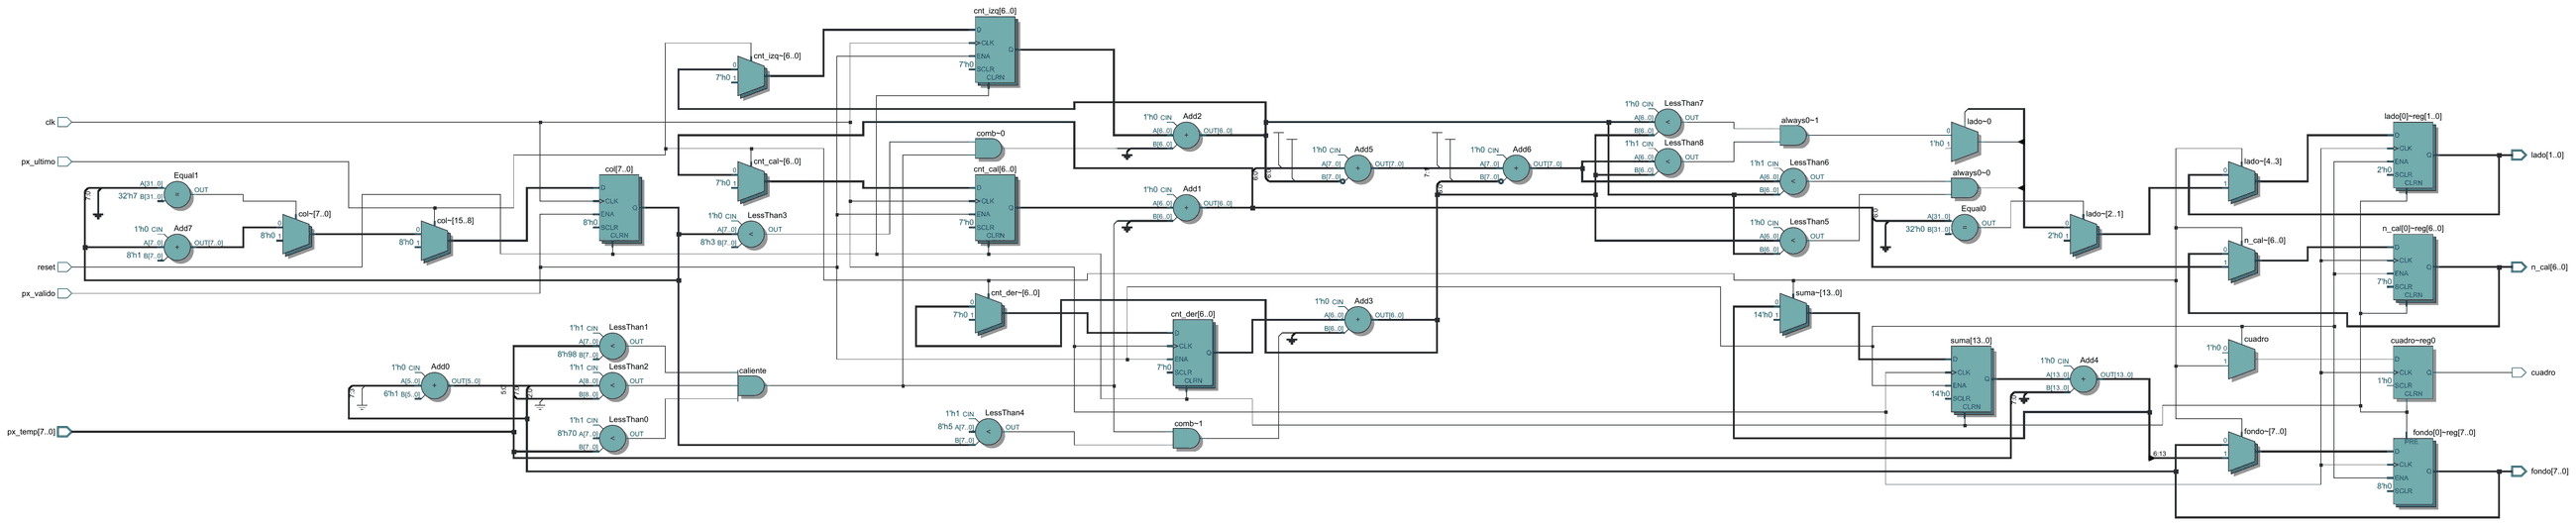
\includegraphics[width=\linewidth]{figs/rtl/rtl_ventana_termica.png}
\caption{El módulo completo.}
\end{subfigure}

\medskip
\begin{subfigure}{0.46\textwidth}
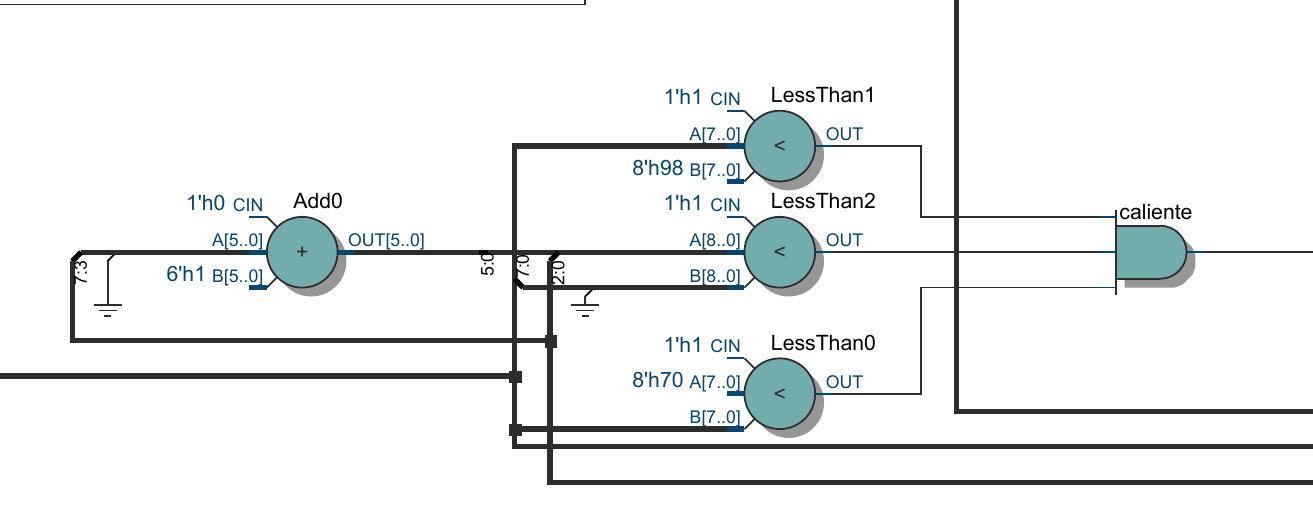
\includegraphics[width=\linewidth]{figs/rtl/zoom_ventana_termica.png}
\caption{Acercamiento: los tres comparadores (\sig{8'h70} = 28~\textdegree C, \sig{8'h98} = 38~\textdegree C y el fondo más 8) y la compuerta \sig{caliente}.}
\end{subfigure}
\caption{\sig{ventana\_termica} en el RTL Viewer de Quartus.}
\label{fig:dventana}
\end{figure}

\modulo{media\_movil4}{hdl/detectores.v}{40 EL, 28 R}
Filtro FIR de cuatro coeficientes iguales (sección~\ref{sec:fir}). Guarda los últimos cuatro conteos en un
registro de corrimiento, los suma con dos bits extra para no desbordar y divide entre cuatro quitando los dos
bits bajos. Quita el vaivén que mete el insecto al caminar.

\modulo{detector\_presencia}{hdl/detectores.v}{9 EL, 4 R}
Compara el conteo filtrado con dos umbrales: \sig{pre} vale 1 con 2 píxeles o más (conviene acercarse) y
\sig{sobre}, con 8 o más. Un contador de 4 bits, que se satura en 15, cuenta los cuadros seguidos con
\sig{sobre} y vuelve a cero en cuanto falta uno; al llegar a cuatro levanta \sig{confirmado}. Así un reflejo de un
solo cuadro no dispara la alerta.

\modulo{detector\_quietud}{hdl/detectores.v}{10 EL, 4 R}
Recibe la «actividad» de la IMU (0 a 255). Si se queda por debajo de 8 durante diez cuadros seguidos, un segundo,
declara quieto al insecto; una sola lectura por arriba baja la salida de inmediato.

\modulo{lfsr16}{hdl/detectores.v}{16 EL, 16 R}
Registro de corrimiento con realimentación, $x^{16}+x^{14}+x^{13}+x^{11}+1$, de periodo 65\,535 y semilla
\sig{0xACE1}. Avanza un paso por cuadro. La política gira al azar cuando sus nueve bits bajos son cero, es decir
una vez cada 512 cuadros (51.2~s) en promedio, y el bit 9 decide el lado.

\modulo{fsm\_politica}{hdl/fsm\_politica.v}{181 EL, 64 R}
Es el control. Un bloque combinacional calcula el estado siguiente y si este cuadro sale un estímulo; un bloque
secuencial lo registra y actualiza los temporizadores, todos en décimas de segundo:
\begin{itemize}
  \item \textbf{REPOSO} espera la orden de arranque. \textbf{EXPLORAR} deja caminar y vigila, en este orden, la
        mancha de calor, el presupuesto, la quietud y el azar.
  \item \textbf{REACTIVAR}: tras 15~s quieto manda un pulso de avance y observa 3~s. Si arranca, la espera vuelve a
        15~s; si no, se duplica hasta 120~s. \textbf{REORIENTAR} gira a un lado al azar y regresa a explorar.
  \item \textbf{ACERCAR}: con \sig{pre} gira hacia el lado de la mancha, o avanza si está quieto; si la pierde 5~s,
        vuelve a explorar. \textbf{CONFIRMAR} deja de estimular y espera \sig{confirmado}. \textbf{ALERTAR} es final y
        emite una baliza cada 5~s. \textbf{DESCANSO} espera a que baje el presupuesto.
\end{itemize}
Entre estímulos pasan al menos 10~s. El presupuesto es una cuenta Q8.8: cada estímulo suma 256 (1.0) y cada 23
cuadros pierde $1/256$ de su valor, al menos una cuenta, lo que da una constante de unos 590~s, cercana a la
recuperación del insecto. Con 12.0 acumulados se deja de estimular. Así se acota la habituación y la carga sobre
el animal sin medir su respuesta.

\modulo{gen\_estimulo}{hdl/gen\_estimulo.v}{64 EL, 47 R}
Con cada \sig{disparo} saca 25 periodos de una onda cuadrada de 50~Hz (0.5~s) por el canal pedido: avance,
izquierda o derecha. Un contador mide el medio periodo (500\,000 ciclos a 50~MHz) y un bit alterna las mitades.
Cada canal tiene dos salidas en contrafase, \sig{fase\_a} y \sig{fase\_b}, que en un par de electrodos dan una
onda bifásica sin componente continua; para la luz ultravioleta basta \sig{led\_on}. Mientras hay un tren en
curso ignora otros disparos, y todas las salidas son registros para no tener transitorios.

\modulo{nucleo\_biobot}{hdl/nucleo\_biobot.v}{477 EL, 224 R}
Conecta los siete módulos. No depende de la tarjeta: recibe píxeles ya separados y la actividad, y entrega las
fases, el estado, la alerta, la baliza y la telemetría. Es el mismo archivo en la demostración, en la red de tres
tarjetas (donde la ventana se ajusta a 35--38~\textdegree C por parámetros) y en el layout. La
figura~\ref{fig:rtlnucleo} es lo que Quartus entiende de él.

\begin{figure}[!htb]
\centering
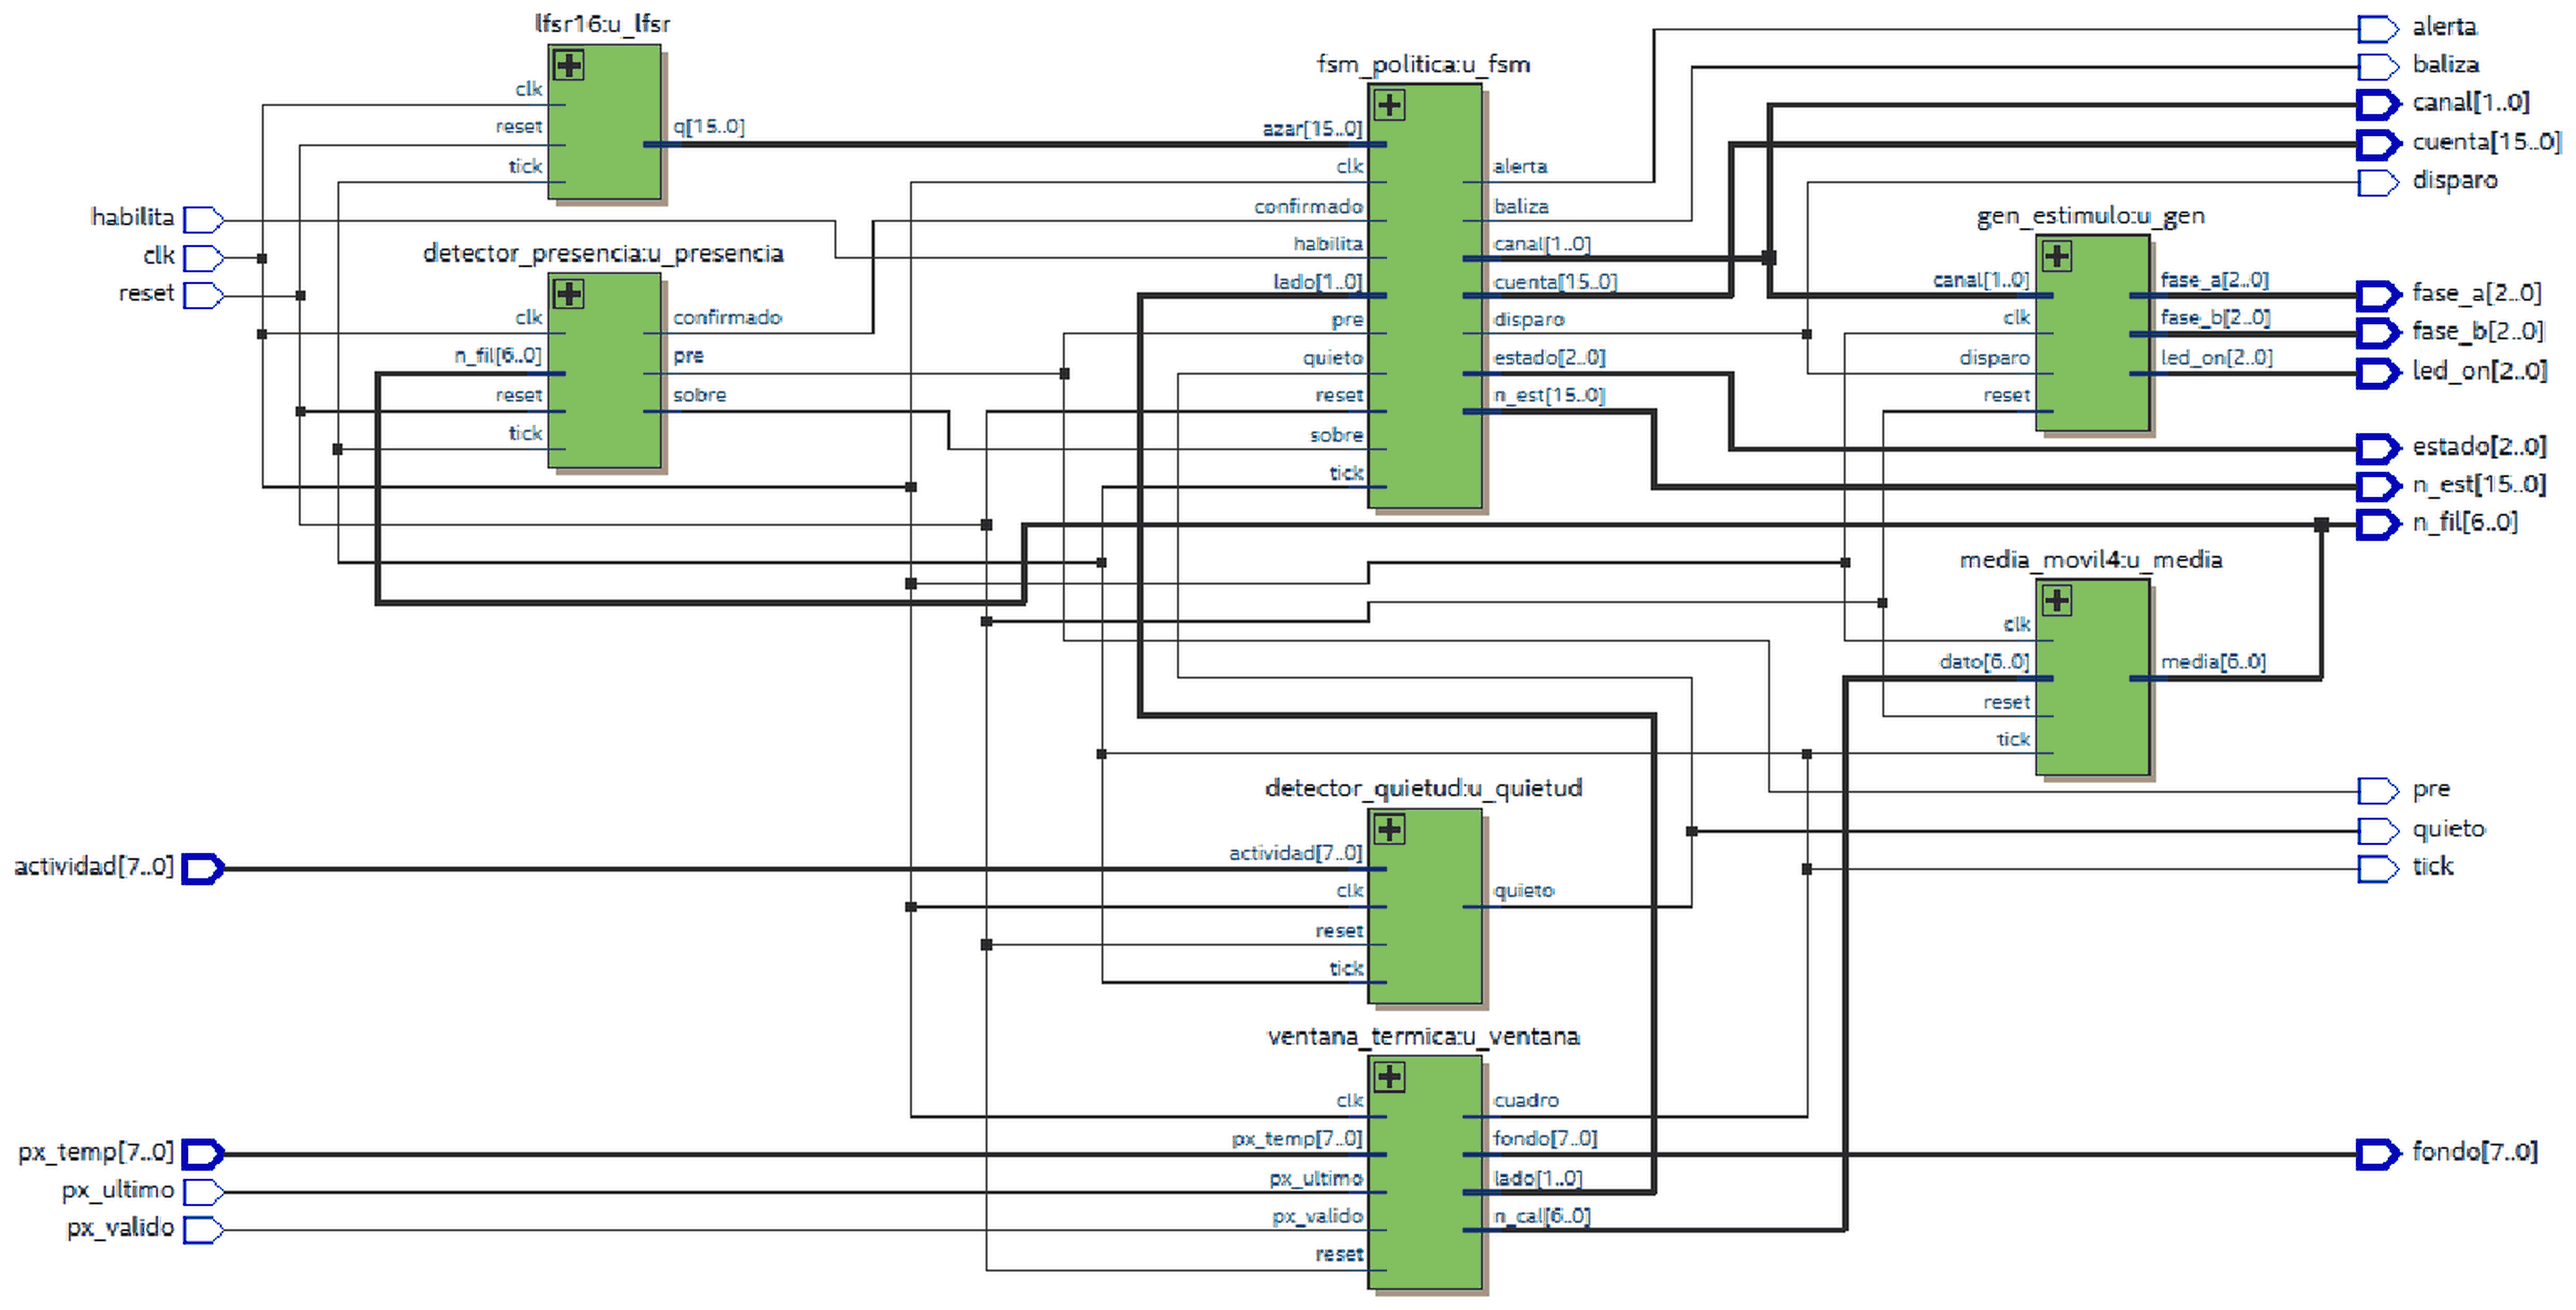
\includegraphics[width=0.94\textwidth]{figs/rtl/rtl_nucleo.png}
\caption{\sig{nucleo\_biobot} en el RTL Viewer de Quartus: los siete módulos y sus conexiones.}
\label{fig:rtlnucleo}
\end{figure}

\subsubsection{Enlace serie del prototipo}

\modulo{uart\_rx}{hdl/uart\_rx.v}{63 EL, 40 R}
Receptor 8N1 de la práctica~4. Dos flip-flops sincronizan la línea; al ver el flanco de bajada espera medio bit y
confirma que el bit de inicio sigue en 0 (si no, fue ruido y lo descarta). Desde ahí cuenta bits completos
(5\,208 ciclos a 9\,600 baudios o 434 a 115\,200) y muestrea cada dato en su centro, empezando por el menos
significativo. En el centro del bit de paro entrega el byte con un pulso \sig{data\_valid}
(figura~\ref{fig:duart}).

\begin{figure}[!htb]
\centering
\begin{tikzpicture}[x=1.22cm,y=0.75cm,every node/.style={font=\scriptsize}]
\draw[thick,Primary] (-0.8,1) -- (0,1) -- (0,0) -- (1,0);
\foreach \i in {1,...,8} {\draw[thick,Primary] (\i,0) rectangle (\i+1,1); \node at (\i+0.5,1.35) {$d_{\the\numexpr\i-1\relax}$};}
\draw[thick,Primary] (9,0) -- (9,1) -- (10.6,1);
\node at (0.5,1.35) {inicio}; \node at (9.6,1.35) {paro}; \node at (-0.55,1.35) {reposo};
\foreach \i in {0,...,9} {\draw[Accent,very thick,-{Stealth[length=1.6mm]}] (\i+0.5,-0.85) -- (\i+0.5,-0.1);}
\draw[<->,Secondary] (0,-0.35) -- (0.5,-0.35); \node[Secondary] at (0.1,-0.75) {$\tfrac12$ bit};
\draw[<->,Secondary] (2.5,-0.35) -- (3.5,-0.35); \node[Secondary] at (3,-0.75) {1 bit};
\node[Accent] at (5,-1.2) {muestreo en el centro de cada bit; en el de paro sale \sig{data\_valid}};
\end{tikzpicture}
\caption{Instantes en que \sig{uart\_rx} lee la línea.}
\label{fig:duart}
\end{figure}

\modulo{uart\_tx}{hdl/uart\_tx.v}{43 EL, 31 R}
Con \sig{tx\_start} carga un registro de diez bits, \sig{\{1, dato, 0\}}, y lo recorre a la derecha un bit por
periodo. Mientras transmite, \sig{busy} vale 1 y no acepta otra petición.

\modulo{receptor\_trama}{hdl/enlace\_serie.v}{86 EL, 58 R}
Arma un cuadro con los bytes que llegan: \sig{0xA5}, actividad y 64 píxeles. La actividad va primero para que esté
estable cuando el último píxel cierra el cuadro. Si pasan 5~ms sin bytes, abandona la trama y vuelve a buscar la
cabecera.

\modulo{emisor\_estado}{hdl/enlace\_serie.v}{31 EL, 16 R}
Después de cada cuadro contesta cuatro bytes: \sig{0x5A}; alerta, estado, si hubo estímulo, canal y quietud;
\sig{pre} y conteo filtrado; y la parte entera del presupuesto. Espera tres ciclos tras el \sig{tick} para leer el
estado ya actualizado y guarda el disparo en un bit para no perderlo entre reportes.

\subsubsection{Verificación contra un modelo de referencia}

Antes de escribir el Verilog se programó en Python un modelo que hace las mismas cuentas con enteros, registro por
registro. Genera los cuadros de prueba y la respuesta esperada, y los bancos comparan cuadro por cuadro
(tabla~\ref{tab:bancos}). El prototipo completo ocupa 722~EL y 372~R, con $f_{\max}=72.08$~MHz.

\begin{table}[!htb]
\centering\footnotesize
\caption{Resultados de simulación del núcleo con Icarus Verilog 12.}
\label{tab:bancos}
\rowcolors{2}{SoftGray}{white}
\begin{tabularx}{\textwidth}{@{}>{\ttfamily\raggedright\arraybackslash}p{2.7cm} >{\raggedright\arraybackslash}X >{\raggedright\arraybackslash}p{5.0cm}@{}}
\toprule
\rowcolor{TableHead} \normalfont\textbf{Banco} & \textbf{Qué prueba} & \textbf{Resultado} \\
\midrule
tb\_nucleo & Pausas, insecto que no responde, acercamiento, ambiente a 30 y 37.5~\textdegree C, objeto a 47.5~\textdegree C y 3\,000 cuadros al azar & 11\,424 de 11\,424 cuadros coinciden; se visitan los ocho estados \\
tb\_gen\_estimulo & Periodo, ciclo, duración, fases y disparo a medio tren & 3 de 3 trenes: 25 periodos de 20.000~ms \\
tb\_top & Sistema completo por UART hasta la detección & 500 de 500 respuestas coinciden \\
tb\_demo & Núcleo e insecto de prueba en el mismo chip & 4 de 4: alerta solo con persona, cuadro 558 \\
tb\_dos\_tarjetas & Dos tarjetas unidas solo por UART & 2 de 2: alerta en el cuadro 557 \\
\bottomrule
\end{tabularx}
\end{table}
